\documentclass{standalone}
\usepackage{tikz}
\usetikzlibrary{patterns, positioning}

\begin{document}
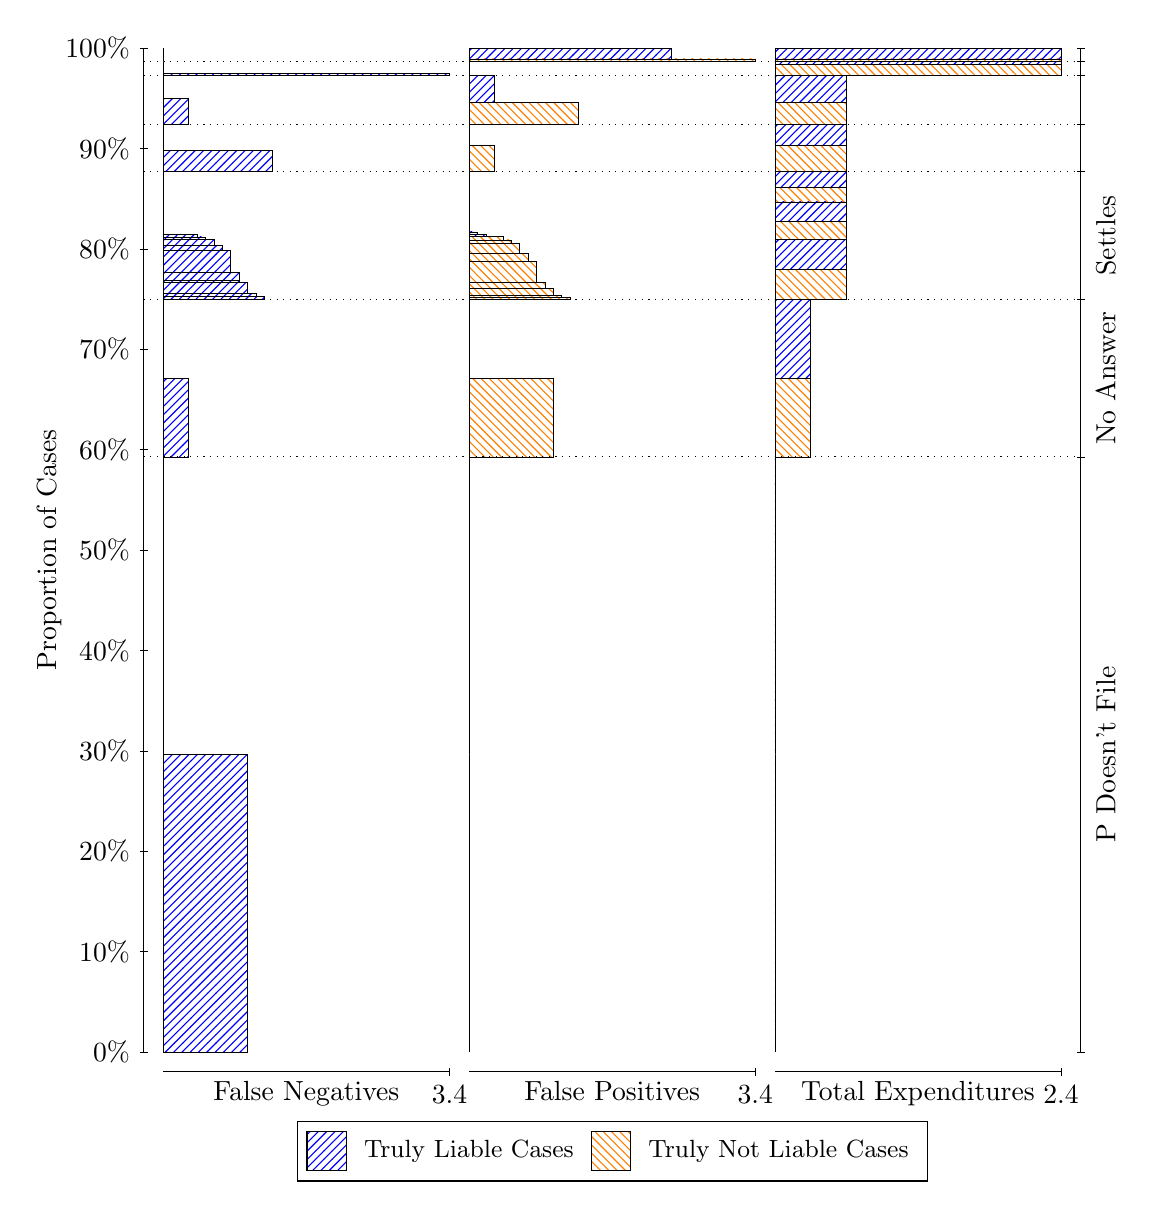
\begin{tikzpicture}
\draw[black, very thin] (1.5,1.75) -- (1.5,14.5);
\node[rotate=90, anchor=center] at (0.3, 8.125) {Proportion of Cases};
\draw[black, very thin] (1.45,1.75) -- (1.55,1.75);
\node[anchor=east] at (1.45, 1.75) {0\%};
\draw[black, very thin] (1.45,3.025) -- (1.55,3.025);
\node[anchor=east] at (1.45, 3.025) {10\%};
\draw[black, very thin] (1.45,4.3) -- (1.55,4.3);
\node[anchor=east] at (1.45, 4.3) {20\%};
\draw[black, very thin] (1.45,5.575) -- (1.55,5.575);
\node[anchor=east] at (1.45, 5.575) {30\%};
\draw[black, very thin] (1.45,6.85) -- (1.55,6.85);
\node[anchor=east] at (1.45, 6.85) {40\%};
\draw[black, very thin] (1.45,8.125) -- (1.55,8.125);
\node[anchor=east] at (1.45, 8.125) {50\%};
\draw[black, very thin] (1.45,9.4) -- (1.55,9.4);
\node[anchor=east] at (1.45, 9.4) {60\%};
\draw[black, very thin] (1.45,10.675) -- (1.55,10.675);
\node[anchor=east] at (1.45, 10.675) {70\%};
\draw[black, very thin] (1.45,11.95) -- (1.55,11.95);
\node[anchor=east] at (1.45, 11.95) {80\%};
\draw[black, very thin] (1.45,13.225) -- (1.55,13.225);
\node[anchor=east] at (1.45, 13.225) {90\%};
\draw[black, very thin] (1.45,14.5) -- (1.55,14.5);
\node[anchor=east] at (1.45, 14.5) {100\%};

\draw[black, very thin] (13.4,1.75) -- (13.4,14.5);
\draw[black, very thin] (13.35,1.75) -- (13.45,1.75);
\node[anchor=west] at (13.35, 1.75) {};
\draw[black, very thin] (13.35,9.3072) -- (13.45,9.3072);
\node[anchor=west] at (13.35, 9.3072) {};
\draw[black, very thin] (13.35,11.303) -- (13.45,11.303);
\node[anchor=west] at (13.35, 11.303) {};
\draw[black, very thin] (13.35,12.934) -- (13.45,12.934);
\node[anchor=west] at (13.35, 12.934) {};
\draw[black, very thin] (13.35,13.531) -- (13.45,13.531);
\node[anchor=west] at (13.35, 13.531) {};
\draw[black, very thin] (13.35,14.148) -- (13.45,14.148);
\node[anchor=west] at (13.35, 14.148) {};
\draw[black, very thin] (13.35,14.329) -- (13.45,14.329);
\node[anchor=west] at (13.35, 14.329) {};
\draw[black, very thin] (13.35,14.5) -- (13.45,14.5);
\node[anchor=west] at (13.35, 14.5) {};

\draw[black, very thin, pattern color=blue, pattern=north east lines] (1.75,1.75) rectangle (2.8186,5.5285);
\draw[black, very thin, pattern color=orange, pattern=north west lines] (1.75,5.5285) rectangle (1.75,9.3072);
\draw[black, very thin, pattern color=blue, pattern=north east lines] (1.75,9.3072) rectangle (2.0706,10.305);
\draw[black, very thin, pattern color=orange, pattern=north west lines] (1.75,10.305) rectangle (1.75,11.303);
\draw[black, very thin, pattern color=blue, pattern=north east lines] (1.75,11.303) rectangle (3.0324,11.342);
\draw[black, very thin, pattern color=blue, pattern=north east lines] (1.75,11.342) rectangle (2.9255,11.382);
\draw[black, very thin, pattern color=blue, pattern=north east lines] (1.75,11.382) rectangle (2.8186,11.525);
\draw[black, very thin, pattern color=blue, pattern=north east lines] (1.75,11.525) rectangle (2.7118,11.545);
\draw[black, very thin, pattern color=blue, pattern=north east lines] (1.75,11.545) rectangle (2.7118,11.648);
\draw[black, very thin, pattern color=blue, pattern=north east lines] (1.75,11.648) rectangle (2.6049,11.927);
\draw[black, very thin, pattern color=blue, pattern=north east lines] (1.75,11.927) rectangle (2.498,11.994);
\draw[black, very thin, pattern color=blue, pattern=north east lines] (1.75,11.994) rectangle (2.3912,12.071);
\draw[black, very thin, pattern color=blue, pattern=north east lines] (1.75,12.071) rectangle (2.2843,12.101);
\draw[black, very thin, pattern color=blue, pattern=north east lines] (1.75,12.101) rectangle (2.1775,12.129);
\draw[black, very thin, pattern color=orange, pattern=north west lines] (1.75,12.129) rectangle (1.75,12.934);
\draw[black, very thin, pattern color=blue, pattern=north east lines] (1.75,12.934) rectangle (3.1392,13.201);
\draw[black, very thin, pattern color=orange, pattern=north west lines] (1.75,13.201) rectangle (1.75,13.531);
\draw[black, very thin, pattern color=blue, pattern=north east lines] (1.75,13.531) rectangle (2.0706,13.865);
\draw[black, very thin, pattern color=orange, pattern=north west lines] (1.75,13.865) rectangle (1.75,14.148);
\draw[black, very thin, pattern color=blue, pattern=north east lines] (1.75,14.148) rectangle (5.3833,14.181);
\draw[black, very thin, pattern color=orange, pattern=north west lines] (1.75,14.181) rectangle (1.75,14.329);
\draw[black, very thin, pattern color=orange, pattern=north west lines] (1.75,14.329) rectangle (1.75,14.362);
\draw[black, very thin, pattern color=blue, pattern=north east lines] (1.75,14.362) rectangle (1.75,14.5);
\draw[black, very thin, pattern color=orange, pattern=north west lines] (5.6333,1.75) rectangle (5.6333,5.5286);
\draw[black, very thin, pattern color=blue, pattern=north east lines] (5.6333,5.5286) rectangle (5.6333,9.3072);
\draw[black, very thin, pattern color=orange, pattern=north west lines] (5.6333,9.3072) rectangle (6.702,10.305);
\draw[black, very thin, pattern color=blue, pattern=north east lines] (5.6333,10.305) rectangle (5.6333,11.303);
\draw[black, very thin, pattern color=orange, pattern=north west lines] (5.6333,11.303) rectangle (6.9157,11.333);
\draw[black, very thin, pattern color=orange, pattern=north west lines] (5.6333,11.333) rectangle (6.8088,11.363);
\draw[black, very thin, pattern color=orange, pattern=north west lines] (5.6333,11.363) rectangle (6.702,11.45);
\draw[black, very thin, pattern color=orange, pattern=north west lines] (5.6333,11.45) rectangle (6.5951,11.528);
\draw[black, very thin, pattern color=orange, pattern=north west lines] (5.6333,11.528) rectangle (6.4882,11.793);
\draw[black, very thin, pattern color=orange, pattern=north west lines] (5.6333,11.793) rectangle (6.3814,11.896);
\draw[black, very thin, pattern color=orange, pattern=north west lines] (5.6333,11.896) rectangle (6.2745,12.021);
\draw[black, very thin, pattern color=orange, pattern=north west lines] (5.6333,12.021) rectangle (6.1676,12.064);
\draw[black, very thin, pattern color=orange, pattern=north west lines] (5.6333,12.064) rectangle (6.0608,12.108);
\draw[black, very thin, pattern color=blue, pattern=north east lines] (5.6333,12.108) rectangle (5.8471,12.136);
\draw[black, very thin, pattern color=blue, pattern=north east lines] (5.6333,12.136) rectangle (5.7402,12.166);
\draw[black, very thin, pattern color=blue, pattern=north east lines] (5.6333,12.166) rectangle (5.6333,12.934);
\draw[black, very thin, pattern color=orange, pattern=north west lines] (5.6333,12.934) rectangle (5.9539,13.263);
\draw[black, very thin, pattern color=blue, pattern=north east lines] (5.6333,13.263) rectangle (5.6333,13.531);
\draw[black, very thin, pattern color=orange, pattern=north west lines] (5.6333,13.531) rectangle (7.0225,13.813);
\draw[black, very thin, pattern color=blue, pattern=north east lines] (5.6333,13.813) rectangle (5.9539,14.148);
\draw[black, very thin, pattern color=orange, pattern=north west lines] (5.6333,14.148) rectangle (5.6333,14.296);
\draw[black, very thin, pattern color=blue, pattern=north east lines] (5.6333,14.296) rectangle (5.6333,14.329);
\draw[black, very thin, pattern color=orange, pattern=north west lines] (5.6333,14.329) rectangle (9.2667,14.362);
\draw[black, very thin, pattern color=blue, pattern=north east lines] (5.6333,14.362) rectangle (8.198,14.5);
\draw[black, very thin, pattern color=orange, pattern=north west lines] (9.5167,1.75) rectangle (9.5167,5.5286);
\draw[black, very thin, pattern color=blue, pattern=north east lines] (9.5167,5.5286) rectangle (9.5167,9.3072);
\draw[black, very thin, pattern color=orange, pattern=north west lines] (9.5167,9.3072) rectangle (9.9708,10.305);
\draw[black, very thin, pattern color=blue, pattern=north east lines] (9.5167,10.305) rectangle (9.9708,11.303);
\draw[black, very thin, pattern color=orange, pattern=north west lines] (9.5167,11.303) rectangle (10.425,11.685);
\draw[black, very thin, pattern color=blue, pattern=north east lines] (9.5167,11.685) rectangle (10.425,12.07);
\draw[black, very thin, pattern color=orange, pattern=north west lines] (9.5167,12.07) rectangle (10.425,12.303);
\draw[black, very thin, pattern color=blue, pattern=north east lines] (9.5167,12.303) rectangle (10.425,12.545);
\draw[black, very thin, pattern color=orange, pattern=north west lines] (9.5167,12.545) rectangle (10.425,12.735);
\draw[black, very thin, pattern color=blue, pattern=north east lines] (9.5167,12.735) rectangle (10.425,12.934);
\draw[black, very thin, pattern color=orange, pattern=north west lines] (9.5167,12.934) rectangle (10.425,13.263);
\draw[black, very thin, pattern color=blue, pattern=north east lines] (9.5167,13.263) rectangle (10.425,13.531);
\draw[black, very thin, pattern color=orange, pattern=north west lines] (9.5167,13.531) rectangle (10.425,13.813);
\draw[black, very thin, pattern color=blue, pattern=north east lines] (9.5167,13.813) rectangle (10.425,14.148);
\draw[black, very thin, pattern color=orange, pattern=north west lines] (9.5167,14.148) rectangle (13.15,14.296);
\draw[black, very thin, pattern color=blue, pattern=north east lines] (9.5167,14.296) rectangle (13.15,14.329);
\draw[black, very thin, pattern color=orange, pattern=north west lines] (9.5167,14.329) rectangle (13.15,14.362);
\draw[black, very thin, pattern color=blue, pattern=north east lines] (9.5167,14.362) rectangle (13.15,14.5);
\draw[black, dotted] (1.5,9.3072) -- (13.4,9.3072);
\draw[black, dotted] (1.5,11.303) -- (13.4,11.303);
\draw[black, dotted] (1.5,12.934) -- (13.4,12.934);
\draw[black, dotted] (1.5,13.531) -- (13.4,13.531);
\draw[black, dotted] (1.5,14.148) -- (13.4,14.148);
\draw[black, dotted] (1.5,14.329) -- (13.4,14.329);
\draw[black, very thin] (1.75,1.5) -- (5.3833,1.5);
\node[anchor=north] at (3.5667, 1.5) {False Negatives};
\draw[black, very thin] (5.3833,1.45) -- (5.3833,1.55);
\node[anchor=north] at (5.3833, 1.45) {3.4};

\draw[black, very thin] (5.6333,1.5) -- (9.2667,1.5);
\node[anchor=north] at (7.45, 1.5) {False Positives};
\draw[black, very thin] (9.2667,1.45) -- (9.2667,1.55);
\node[anchor=north] at (9.2667, 1.45) {3.4};

\draw[black, very thin] (9.5167,1.5) -- (13.15,1.5);
\node[anchor=north] at (11.333, 1.5) {Total Expenditures};
\draw[black, very thin] (13.15,1.45) -- (13.15,1.55);
\node[anchor=north] at (13.15, 1.45) {2.4};

\node[black, centered, rotate=90] at (13.72, 5.5286) {P Doesn't File};
\node[black, centered, rotate=90] at (13.72, 10.305) {No Answer};
\node[black, centered, rotate=90] at (13.72, 12.119) {Settles};





\draw (7.449999999999999,1.5) node[draw=none] (baseCoordinate) {};
\begin{scope}[align=center]
        \matrix[scale=0.5, draw=black, below=0.5cm of baseCoordinate, nodes={draw}, column sep=0.1cm]{
            \node[rectangle, draw, minimum width=0.5cm, minimum height=0.5cm, pattern=north east lines, pattern color=blue] {}; &
            \node[draw=none, font=\small] (B) {Truly Liable Cases}; &
            \node[rectangle, draw, minimum width=0.5cm, minimum height=0.5cm, pattern=north west lines, pattern color=orange] {}; &
            \node[draw=none, font=\small] (B) {Truly Not Liable Cases}; \\
            };
\end{scope}

\end{tikzpicture}
\end{document}